\chapter{Related Work}\label{sec:related_work}
Since the very beginning, the SmartNotes application has been aiming to use the best available solutions and make advantage of other related projects. In this chapter, the reader will find an overview of popular notes taking applications, understand the basis of Version Control Systems, and learn about more technical sections regarding the popular programming languages including Python as well as terms of scalability in a Google App Engine product.

\section{Popular notes taking applications}\label{sec:popular_apps} 
No matter if the user works on a small task like plan a holiday or whether they prepare a list of ideas which they aim to share secretly with their coworkers, a computer application will be a useful help.     

Currently, users have a rich variety of notes taking applications to choose from. One group of applications represents the idea of simple user interface which mimics the well known sticky notes or cork board where the notes are not long and relatively easy to find. Flagship representatives of this group are the Sticky Notes, Knotes  or the Stickies\footnote{Sticky Notes used to be the default for notes taking under GNOME, one of the highly popular Linux desktop environments. The Knotes is a substitute for KDE desktop environment. Stickies is a small and handy application which comes with Apple's Mac OS X that has rivals, e.g. SketchBox aiming at the possibilities of customization.}.The above applications offer simple text highlighting, syntax correction and general layout customization. On the other hand, the remaining group of applications has more features to offer, like rich text formatting with broad fonts support and a possibility of embedding multimedia elements and hyperlinks. Moreover, a number of the applications make use of Internet accounts where notes might be edited and tagged. Because of the great diversity among the applications, it seems worth presenting three of them which appear to deserve special attention and the below sections will briefly introduce and compare them.

\subsection{Google Notebook}\label{subsec:google_notebook}
The first application that appears remarkable is Google Notebook, a Google company product\footnote{Google offer a variety of products. Right next to the browser and the Gmail e-mail service, applications like Google Calendar, Google Docs, Picassa Web or YouTube reach more and more users.} open to the end user without charge or special restrictions. It makes use of typical Google design patterns, which makes its usage naturally easy for users familiar with other Google applications. What is more, Google Notebook has a number standard elements like bookmarks and tags, which shorten the search time when notes are kept in groups. Apart from that, the interface has extended WYSIWYG\footnote{WYSIWYG is an acronym for What You See Is What You Get and is used when referring to editors having user friendly interface, operating on a markup language (i.e.. HTML or \TeX) but at the same time allowing the user for manipulation of the output without having sound command of the markup language.} functionality, which makes the rich text formatting user friendly.

For various reasons, users might like to export their notebooks. With Google Notebook this task is said to be easy and the user has three possibilities to do it: export to HTML format, print or export to Google Doc format. What might be considered as even more practical is the opportunity to collaborate on a notebook with other people by marking the notebook as shared and then inviting others to contribute to it by passing a list of emails. This functionality allows for outstanding user experience where the users may share their ideas by working on one notebook simultaneously or separately. Nevertheless, Google was required to implement a simple Version Control System (henceforth VCS) within the feature in order to merge the parts into one piece and thus handle potential conflict situations. To give an example, a conflict might occur when two or more users are editing the same content, i.e. the same sentence, but in different ways which makes further merging impossible. The way the situation is handled by Google is presented in Figure~\ref{fig:google_notebook}. 
\begin{figure}[ht]
\begin{center}
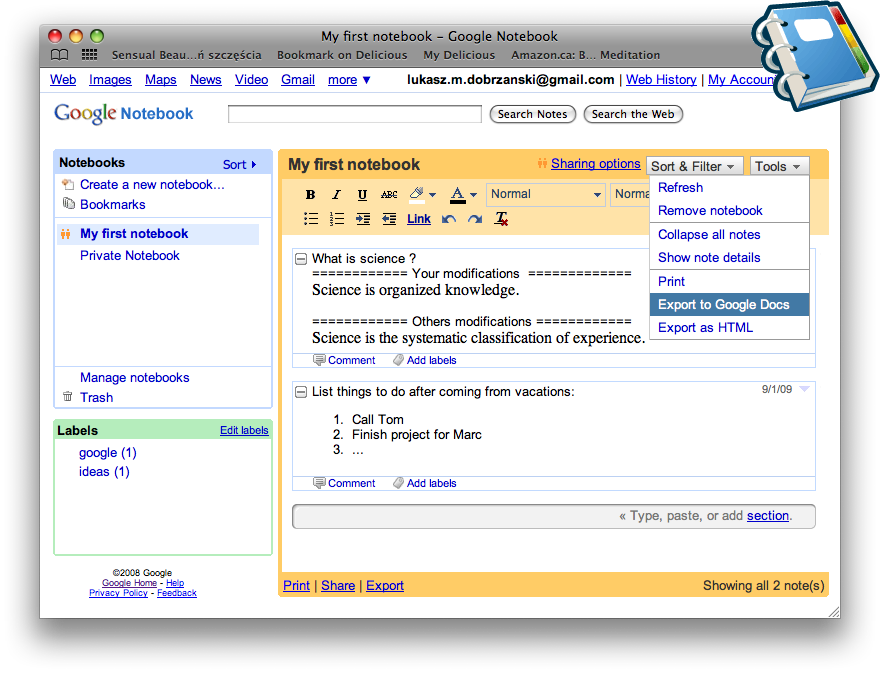
\includegraphics[scale=0.38]{img/google_notebook_demo.png}
\caption{Google Notebook application dealing with conflict situation.}
\label{fig:google_notebook}
\end{center}
\end{figure}
As a result, the user then decides which version is the correct one. The above is only one of the two possibilities that VCS offers in that case. The second one is based on prioritizing performed by the user, where the modification time is registered and the conflict situation is overwritten with the version of the highest priority. All in all, that might appear as an interesting solution, but it also seems that it may lead to mistreating others users' work without an opportunity to notice and react to the conflict.

Finally, what may seem of insignificance importance, but is of huge significance in the light of the dynamic market growth of Internet applications, Google Notebook may be relatively confident of its position. As a matter of fact, already in May 2006 had Google released the initial version of Google Web Toolkit (henceforth GWT), which allowed for huge gains of Java script and CSS compression caring for cross browser compatibility. As a consequence, nowadays GWT is a powerful tool that provides the designer with the opportunity to make the Web-based interface that works as required on a majority of browsers (including mobile devices) available on the market. That may seem even more significant, as the idea of having one's own notebook on mobile devices has a great potential. 

\subsection{Evernote}\label{subsec:evernote}
The second notes taking application that is worth describing is Evernote, which is a commercial product belonging to Evernote Corporation. It has a functional interface, a bunch of unique features and a still growing group of users. Moreover, the application supports multiple mobile devices, like various operating systems, and allows for adding, modifying and grouping notes taken by its users in a swift manner. Further advantages of the application regard the approach to how the notes are made in Evernote. Specifically, the product provides the opportunity to embed various multimedia elements in the notes, which converts the note taking into a process similar to editing a blog entry. Additionally, Evernote allows for clipping all items found on the Internet, from books, through cooking recipes, to interesting articles that the user wills to return to later. To take the argument further, the latter is possible when they use Evernote on the same or another device which has the product installed. It is worth mentioning the fact that this particular feature is especially useful to users dealing with a massive amount of information that cannot be read or memorized straight away and which, thanks to Evernote, may be stored in an easily searchable way. 
\begin{figure}[ht]
\begin{center}
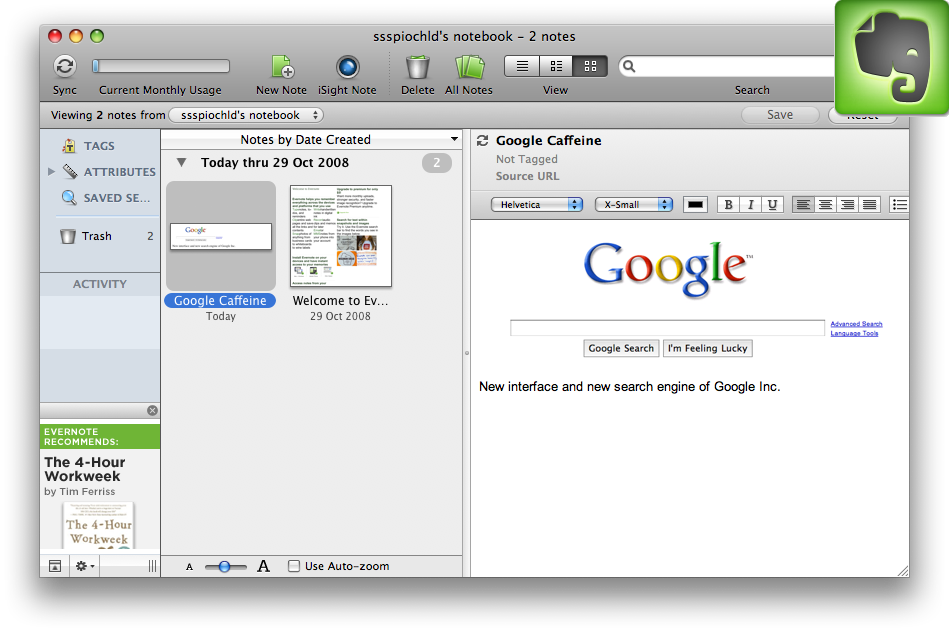
\includegraphics[scale=0.38]{img/evernote_demo.png}
\caption{Evernote application interface layout.}
\label{fig:evernote_demo}
\end{center}
\end{figure}
Yet another distinguished feature of Evernote is that images added to the product are also searchable, which means that text inscribed in the pictures is recognized as any other text, a point in case being a business contact card added to Evernote in couple of seconds by taking its photo, which may be afterwards found by typing in keywords from the card. By taking a photo of a ticket, bill or any other element with text element, Evernote users find it easy to use the elastic tool for importing data to their notes that otherwise would become lost or that would need significantly more time to arrive onto the product in the traditional way.

As mentioned in the beginning of this section, Evernote is a commercial product, which means that its code is proprietary software of Evernote Corporation. It may be used without charge with certain limitations, i.e. no collaboration option, limited file synchronization formats and lower monthly rate of multimedia elements that may be clipped to the application. Not surprisingly, free users are also required to accept typical promotion and advertisement materials in order to use the application. On the other hand, the cost of a premium account with extended options and lower limitations is 5\$ a month or 45\$ for a year, which still remains a reasonable price for such an interesting tool. 

\subsection{Things}\label{subsec:things} 
Things differs from the already introduced applications. It allows for taking notes and supports other task management tools. The idea of Things successfully follows the concept of the GTD\footnote{Get Things Done GTD is a term naming a set of functions allowing user to efficiently organize his work including business arrangements just as shopping lists.} application and that received a couple of awards like Apple Design Award or the Best Of Show award from the Macworld magazine. 
\begin{figure}[ht]
\begin{center}
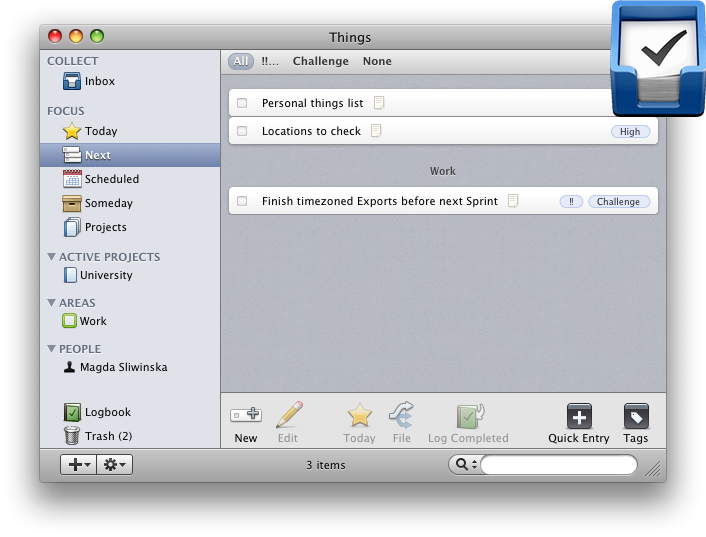
\includegraphics[scale=0.38]{img/things_demo.png}
\caption{Things application interface layout.}
\label{fig:things_demo}
\end{center}
\end{figure}
 
The feature list of the Things application appears impressive and includes the access to such task management tools as:
 \begin{itemize}
 \item{Calendar. Each task can have a due date or repeat the assigned period.}
 \item{Lists of tasks. Easy to manage and edit list with tagging.}
 \item{Projects. Apart from areas of responsibility tasks can be structured in separate projects.}
 \item{Address Book. This feature allows to always have contacts within reach.}
 \item{Daily agenda. This feature allows users to easily orientate what task are scheduled for today.}
 \item{Someday agenda. In contrast to daily agenda, it allows user to browse tasks which do not have any date assigned.}
 \end{itemize}
Yet the above is not everything that Things has to offer. Almost all elements mentioned above can be used in combination and searched easily. Specifically, all the user-defined elements can be reorganized by dragging and dropping, which makes the interface even more functional and improves user experience as the technique appears to be natural for numerous users. Besides, Things makes it possible to import events and tasks from such applications like iCal and iGTD. Additionally, creators of Things have constructed an iPhone-dedicated application which allows to use all of the introduced features and to ensure synchronization between it and the desktop application. 

The Things application, just as Evernote, is a commercial product. When used without buying a license it provides full shareware functionality. The price of a singe user license is 49.95\$, which makes it a competitive offer to Evernote. One clear difference is that the Things application is destined for users of Apple product family like the Mac OS X or the iPhone device.
 
\subsection{Comparison}\label{subsec:vcs_comparison}
The above mentioned programmes represent features with outstanding potential, yet defiantly, they fail to exploit all the features found in applications available on the market. Here, dynamics is an important factor which tends to follow the way users make use of the Internet daily, which should be considered especially when designing any kind of network application targeting an audience of considerable size. Fulfilling the requirements of keeping the speed of market changes and evolving with its users, the applications do not have their market success guaranteed, however, disrespecting the rules might generate a higher cost for the application -- losing all its users. Another rule that seems to be of significant importance is first user experience, which most commonly is built on the perception of the interface. Since currently users enjoy a wide choice of products, it is either the unique features of the application or the interface which trigger interest when users pick a product, which is easily translatable into the decision which application the user decides to use for longer and which they will never open again. Consequently, due to the fact that users naturally tend to have different habits and expectations, a rule of keeping the product as simple as possible supersedes applications with numerous advanced features and a complicated interface and it is this rule that emerges from all rankings of top rated notes taking products. Another conclusion could form a rule that the more a web application mimics the usage of tools that their users could be already used to, the more its chance for success grows. Definitely, one of such confessions for a notes taking application would be note sharing and the possibility to work on notes in smaller groups of contributors. Although a custom solution might be used for the latter, a real Version Control Systems like the one described in Section~\ref{sec:popular_vcs} is used to handle various collaboration scenarios and continuously prove its helpfulness for developers working on projects of various scales. 

\section{Popular Version Control Systems}\label{sec:popular_vcs}
In order to describe VCS, the following scenario has been taken into consideration. A group of developers are working together on a piece of software. Most probably, they divide the work into functional pieces and complete the necessary planning. Afterwards, they begin to code according to their company's coding standards, the approved methodology or favorite schema. Doubtlessly, the developers are required to interact not only by exchanging ideas but also by working on the same parts of code simultaneously and it is at that point when they prefer to be uninterrupted while working on their code, by the same time allowing other developers to track their progress or to make modifications they might find necessary to complete. That basic need was the primary reason for inventing an external software which additionally could inform the developer what changes have been implemented since the last time they worked on the code, a software that merges the wo